%%%%%%%%%%%%%%%%%%%%%%%%%%%%%%%%%%%%%%%%%
% Sullivan Business Report
% LaTeX Template
% Version 1.0 (May 5, 2022)
%
% This template originates from:
% https://www.LaTeXTemplates.com
%
% Author:
% Vel (vel@latextemplates.com)
%
% License:
% CC BY-NC-SA 4.0 (https://creativecommons.org/licenses/by-nc-sa/4.0/)
%
%%%%%%%%%%%%%%%%%%%%%%%%%%%%%%%%%%%%%%%%%


%----------------------------------------------------------------------------------------
%	CLASS, PACKAGES AND OTHER DOCUMENT CONFIGURATIONS
%----------------------------------------------------------------------------------------

\documentclass[
    a4paper, % Paper size, use either a4paper or letterpaper
	12pt, % Default font size, the template is designed to look good at 12pt so it's best not to change this
	%unnumberedsections, % Uncomment for no section numbering
    ]{CSSullivanBusinessReport}
    
    \addbibresource{sample.bib} % BibLaTeX bibliography file

%----------------------------------------------------------------------------------------
%	REPORT INFORMATION
%----------------------------------------------------------------------------------------

\reporttitle{CPE 133 Final Lab} % The report title is to appear on the title page and page headers, do not create manual new lines here as this will carry over to page headers

\reportsubtitle{Robotic Arm\\ with IR input and Servo Output} % Report subtitle, include new lines if needed

\reportauthors{Designed by:\\\smallskip Ethan Vosburg (evosburg@calpoly.edu) \\Wyatt Tack (wtack@calpoly.edu)} % Report authors/group/department, include new lines if needed

\reportdate{\today} % Report date, include new lines for additional information if needed

\rightheadercontent{
\includegraphics[width=3cm]{creodocs_logo.pdf}} % The content in the right header, you may want to add your own company logo or use your company/department name or leave this command empty for no right header content

%----------------------------------------------------------------------------------------

\begin{document}

%----------------------------------------------------------------------------------------
%	TITLE PAGE
%----------------------------------------------------------------------------------------

\thispagestyle{empty} % Suppress headers and footers on this page

\begin{fullwidth} % Use the whole page width
	\vspace*{-0.075\textheight} % Pull logo into the top margin
	
	\hfill
\includegraphics[width=5cm]{creodocs_logo.pdf} % Company logo

	\vspace{0.15\textheight} % Vertical whitespace

	\parbox{0.9\fulltextwidth}{\fontsize{50pt}{52pt}\selectfont\raggedright\textbf{\reporttitle}\par} % Report title, intentionally at less than full width for nice wrapping. Adjust the width of the \parbox and the font size as needed for your title to look good.
	
	\vspace{0.03\textheight} % Vertical whitespace
	
	{\LARGE\textit{\textbf{\reportsubtitle}}\par} % Subtitle
	
	\vfill % Vertical whitespace
	
	{\Large\reportauthors\par} % Report authors, group or department
	
	\vfill\vfill\vfill % Vertical whitespace
	
	{\large\reportdate\par} % Report date
\end{fullwidth}

\newpage

%----------------------------------------------------------------------------------------
%	DISCLAIMER/COPYRIGHT PAGE
%----------------------------------------------------------------------------------------

% \thispagestyle{empty} % Suppress headers and footers on this page

% \begin{twothirdswidth} % Content in this environment to be at two-thirds of the whole page width
% 	\footnotesize % Reduce font size
	
% 	\subsection*{Disclaimer}

% 	Lorem ipsum dolor sit amet, consectetur adipiscing elit. Praesent porttitor arcu luctus, imperdiet urna iaculis, mattis eros. Pellentesque iaculis odio vel nisl ullamcorper, nec faucibus ipsum molestie. Sed dictum nisl non aliquet porttitor. Etiam vulputate arcu dignissim, finibus sem et, viverra nisl. Aenean luctus congue massa, ut laoreet metus ornare in. Nunc fermentum nisi imperdiet lectus tincidunt vestibulum at ac elit.
	
% 	\subsection*{Copyright}
	
% 	\textcopyright~[Year] [Company] 
	
% 	Copyright notice text\ldots In hac habitasse platea dictumst. Curabitur mattis elit sit amet justo luctus vestibulum. In hac habitasse platea dictumst. Pellentesque lobortis justo enim, a condimentum massa tempor eu. Ut quis nulla a quam pretium eleifend nec eu nisl. Nam cursus porttitor eros, sed luctus ligula convallis quis.
	
% 	\subsection*{Contact}
	
% 	Address Line 1\\
% 	Address Line 2\\
% 	Address Line 3
	
% 	Business Number 123456
	
% 	Contact: name@company.com
	
% 	\vfill % Push the following down to the bottom of the page
	
% 	\subsubsection*{Changelog}
	
% 	\scriptsize % Reduce font size further
	
% 	\begin{tabular}{@{} L{0.05\linewidth} L{0.15\linewidth} L{0.6\linewidth} @{}} % Column widths specified here, change as needed for your content
% 		\toprule
% 		v1.0 & 20XX-02-05 & Lorem ipsum dolor sit amet, consectetur adipiscing elit. Praesent porttitor arcu luctus, imperdiet urna iaculis, mattis eros.\\
% 		v1.1 & 20XX-02-27 & Pellentesque iaculis odio vel nisl ullamcorper, nec faucibus ipsum molestie.\\
% 		v1.2 & 20XX-03-15 & Sed dictum nisl non aliquet porttitor.\\
% 		\bottomrule
% 	\end{tabular}
% \end{twothirdswidth}

% \newpage

%----------------------------------------------------------------------------------------
%	TABLE OF CONTENTS
%----------------------------------------------------------------------------------------
\bigskip
\begin{twothirdswidth} % Content in this environment to be at two-thirds of the whole page width
	\tableofcontents % Output the table of contents, automatically generated from the section commands used in the document
\end{twothirdswidth}

\newpage

%----------------------------------------------------------------------------------------
%	SECTIONS
%----------------------------------------------------------------------------------------

\section{Project Description} % Top level section

Our design focused on using a Field Programmable Gate Array to construct an Infrared Remote-Controlled Motorized Arm. Our arm would be controlled by 3 servo motors, allowing for 3 degrees of freedom, which we chose to simulate the Open/Close of the hand, the up and down swivel of the elbow, and the up and down motion of the shoulder/base of the arm. The servo motors would need to be controlled by a module that was capable of taking in the total count of an accumulator and using PWM\sidenote{Pulse Width Modulation} to control the angle that the accumulator total corresponded to. The accumulator would be connected to a series of FSMs\sidenote{Finite State Machines}, that would take the single changing bit from the Infrared sensor and convert it into logic, which would be deciphered by another FSM to determine which button on the remote was pressed and provide either a +1 or a -1\sidenote{through an 8-bit sequence of 2’s complement} to the accumulator storing the total value, corresponding to the angle the specific joint was at.

\section{Design} % Second level section

\subsection{High Level Box Diagram} % Third level section
Our design revolved around one input and three identical outputs. Our main input was the IR Receiver module, which would take data from our remote, running at NEC Protocol. Our three outputs were the PWM lines connected to our 3 servo motors, representing the individual joints on our arm.\sidenote{1 time-dependent input and 3 time-dependent outputs}

% \begin{fullwidth} % Use the whole page width

\begin{figure}[h]
    \centering
    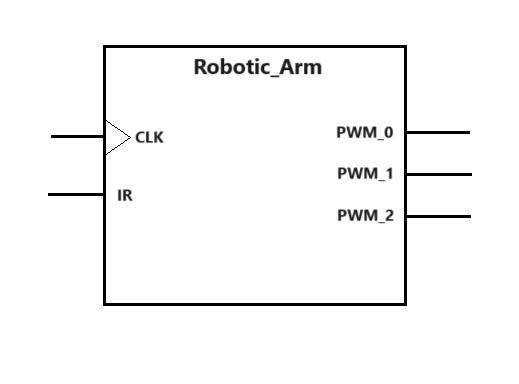
\includegraphics[width=.8\textwidth]{Figures/HLBBD.png}
    \caption[center]{High-Level Black Box Diagram}
    \label{fig:highlevelblockdiagram}
\end{figure}


    \begin{figure}[h]
        \centering
        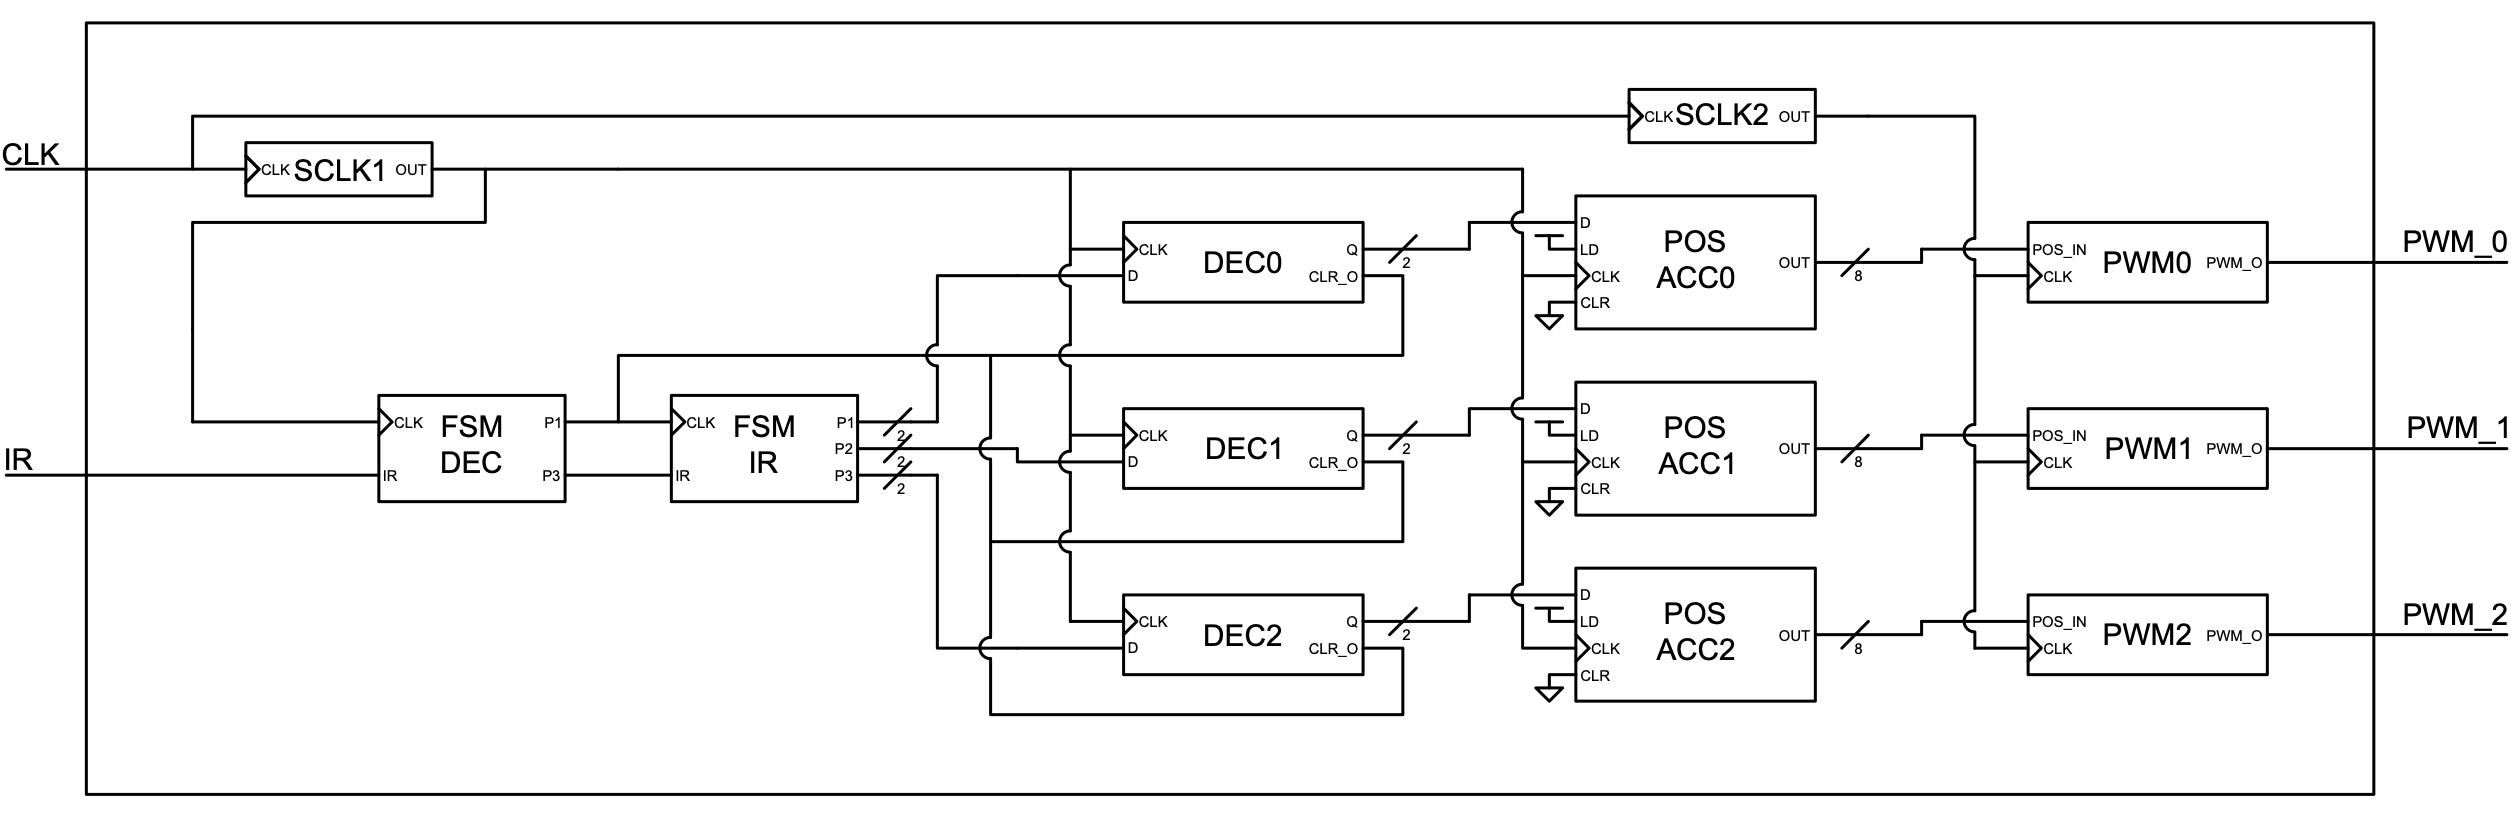
\includegraphics[width=.8\pdfpagewidth]{Figures/High Level Diagram V2.png}
        \caption{Low Level Structural Diagram}
        \label{fig:lowlevelblockdiagram}
    \end{figure}
    
    Our lower-level design consisted of 13 individual modules. Our design comprised of a linear flow of data, with the IR decoding section being made of 2 FSMs and a slow clock, the angle storage line, being comprised of 3 sets of a modified accumulator and a decoder module, and the PWM line comprised of another slow clock and 3 sets of PWM outputting modules for the servo motors. 
    
    \begin{figure}[h]
        \centering
        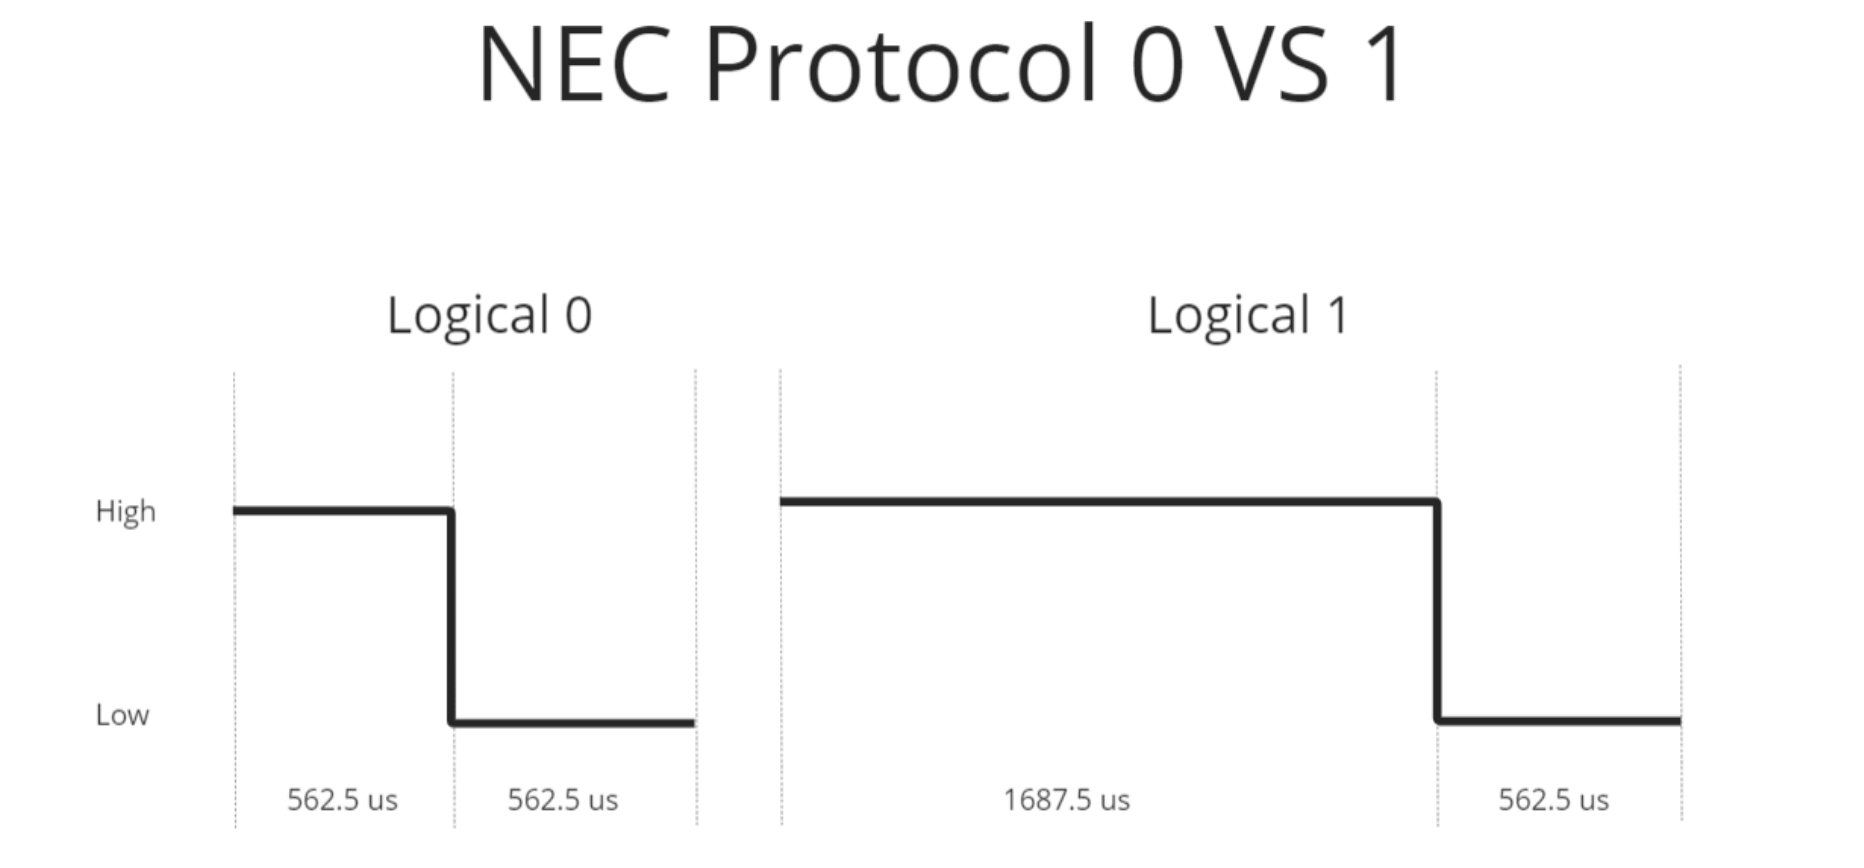
\includegraphics[width=.8\textwidth]{Figures/NEC Protocol.png}
        \caption{Low Level Structural Diagram}
        \label{fig:lowlevelblockdiagram}
    \end{figure}

    Along with each bitstream being a long low pulse and a shorter high pulse before 8 bits of 0 then 8 bits of 1 as a header, then the actual stream of bits is received. For instance, below is shown the oscilloscope output of the IR receiver module when the VOL+ button is pressed on the remote, which would output a long header of 8 logical 0s, 8 logical 1s, and then the hexadecimal code of 0x629D would be Displayed.

    \begin{figure}[h]
        \centering
        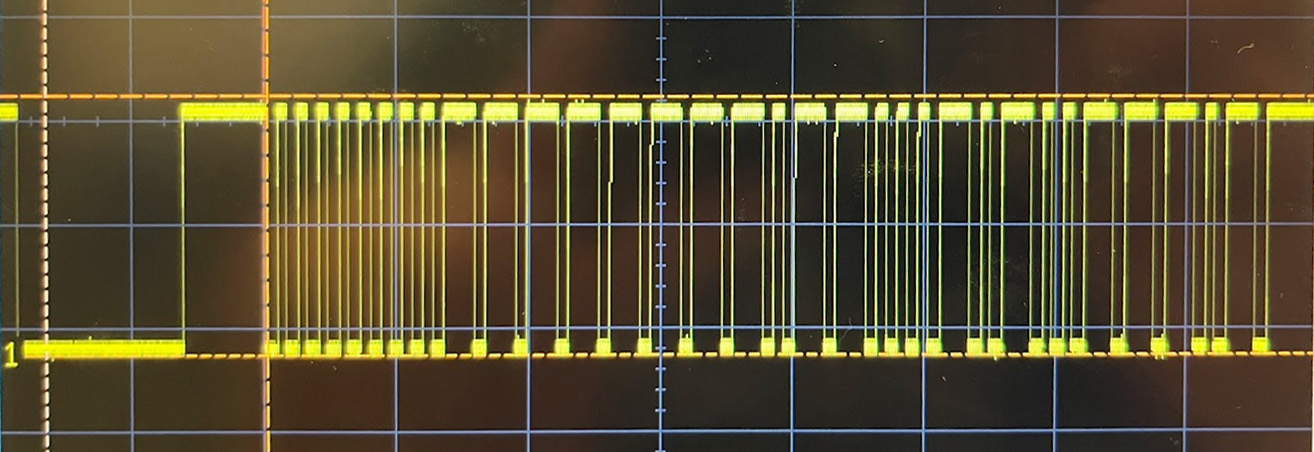
\includegraphics[width=.8\textwidth]{Figures/Oscope Capture.jpg}
        \caption{Oscilloscope Output of VOL+ button on IR Receiver Module}
        \label{fig:lowlevelblockdiagram}
    \end{figure}

    \newpage
    Our first FSM would take in the stream of bits, and output a 0 and a clock pulse when the stream for 0 was detected, or a 1 and a clock pulse when the stream for 1 is detected. The second FSM ran off the clock and output bit from the first FSM, and would take in each bit to determine which 16 bit long code the stream output to with each button press, and if the stream aligned with one of the buttons we chose, the state machine would output either a logical +1 or -1 (in 2’s complement for 2 bits) at one of the 3 ports, corresponding to which servo the button pressed was meant to control. Both FSM state diagrams are shown below.

    \begin{figure}[h]
        \centering
        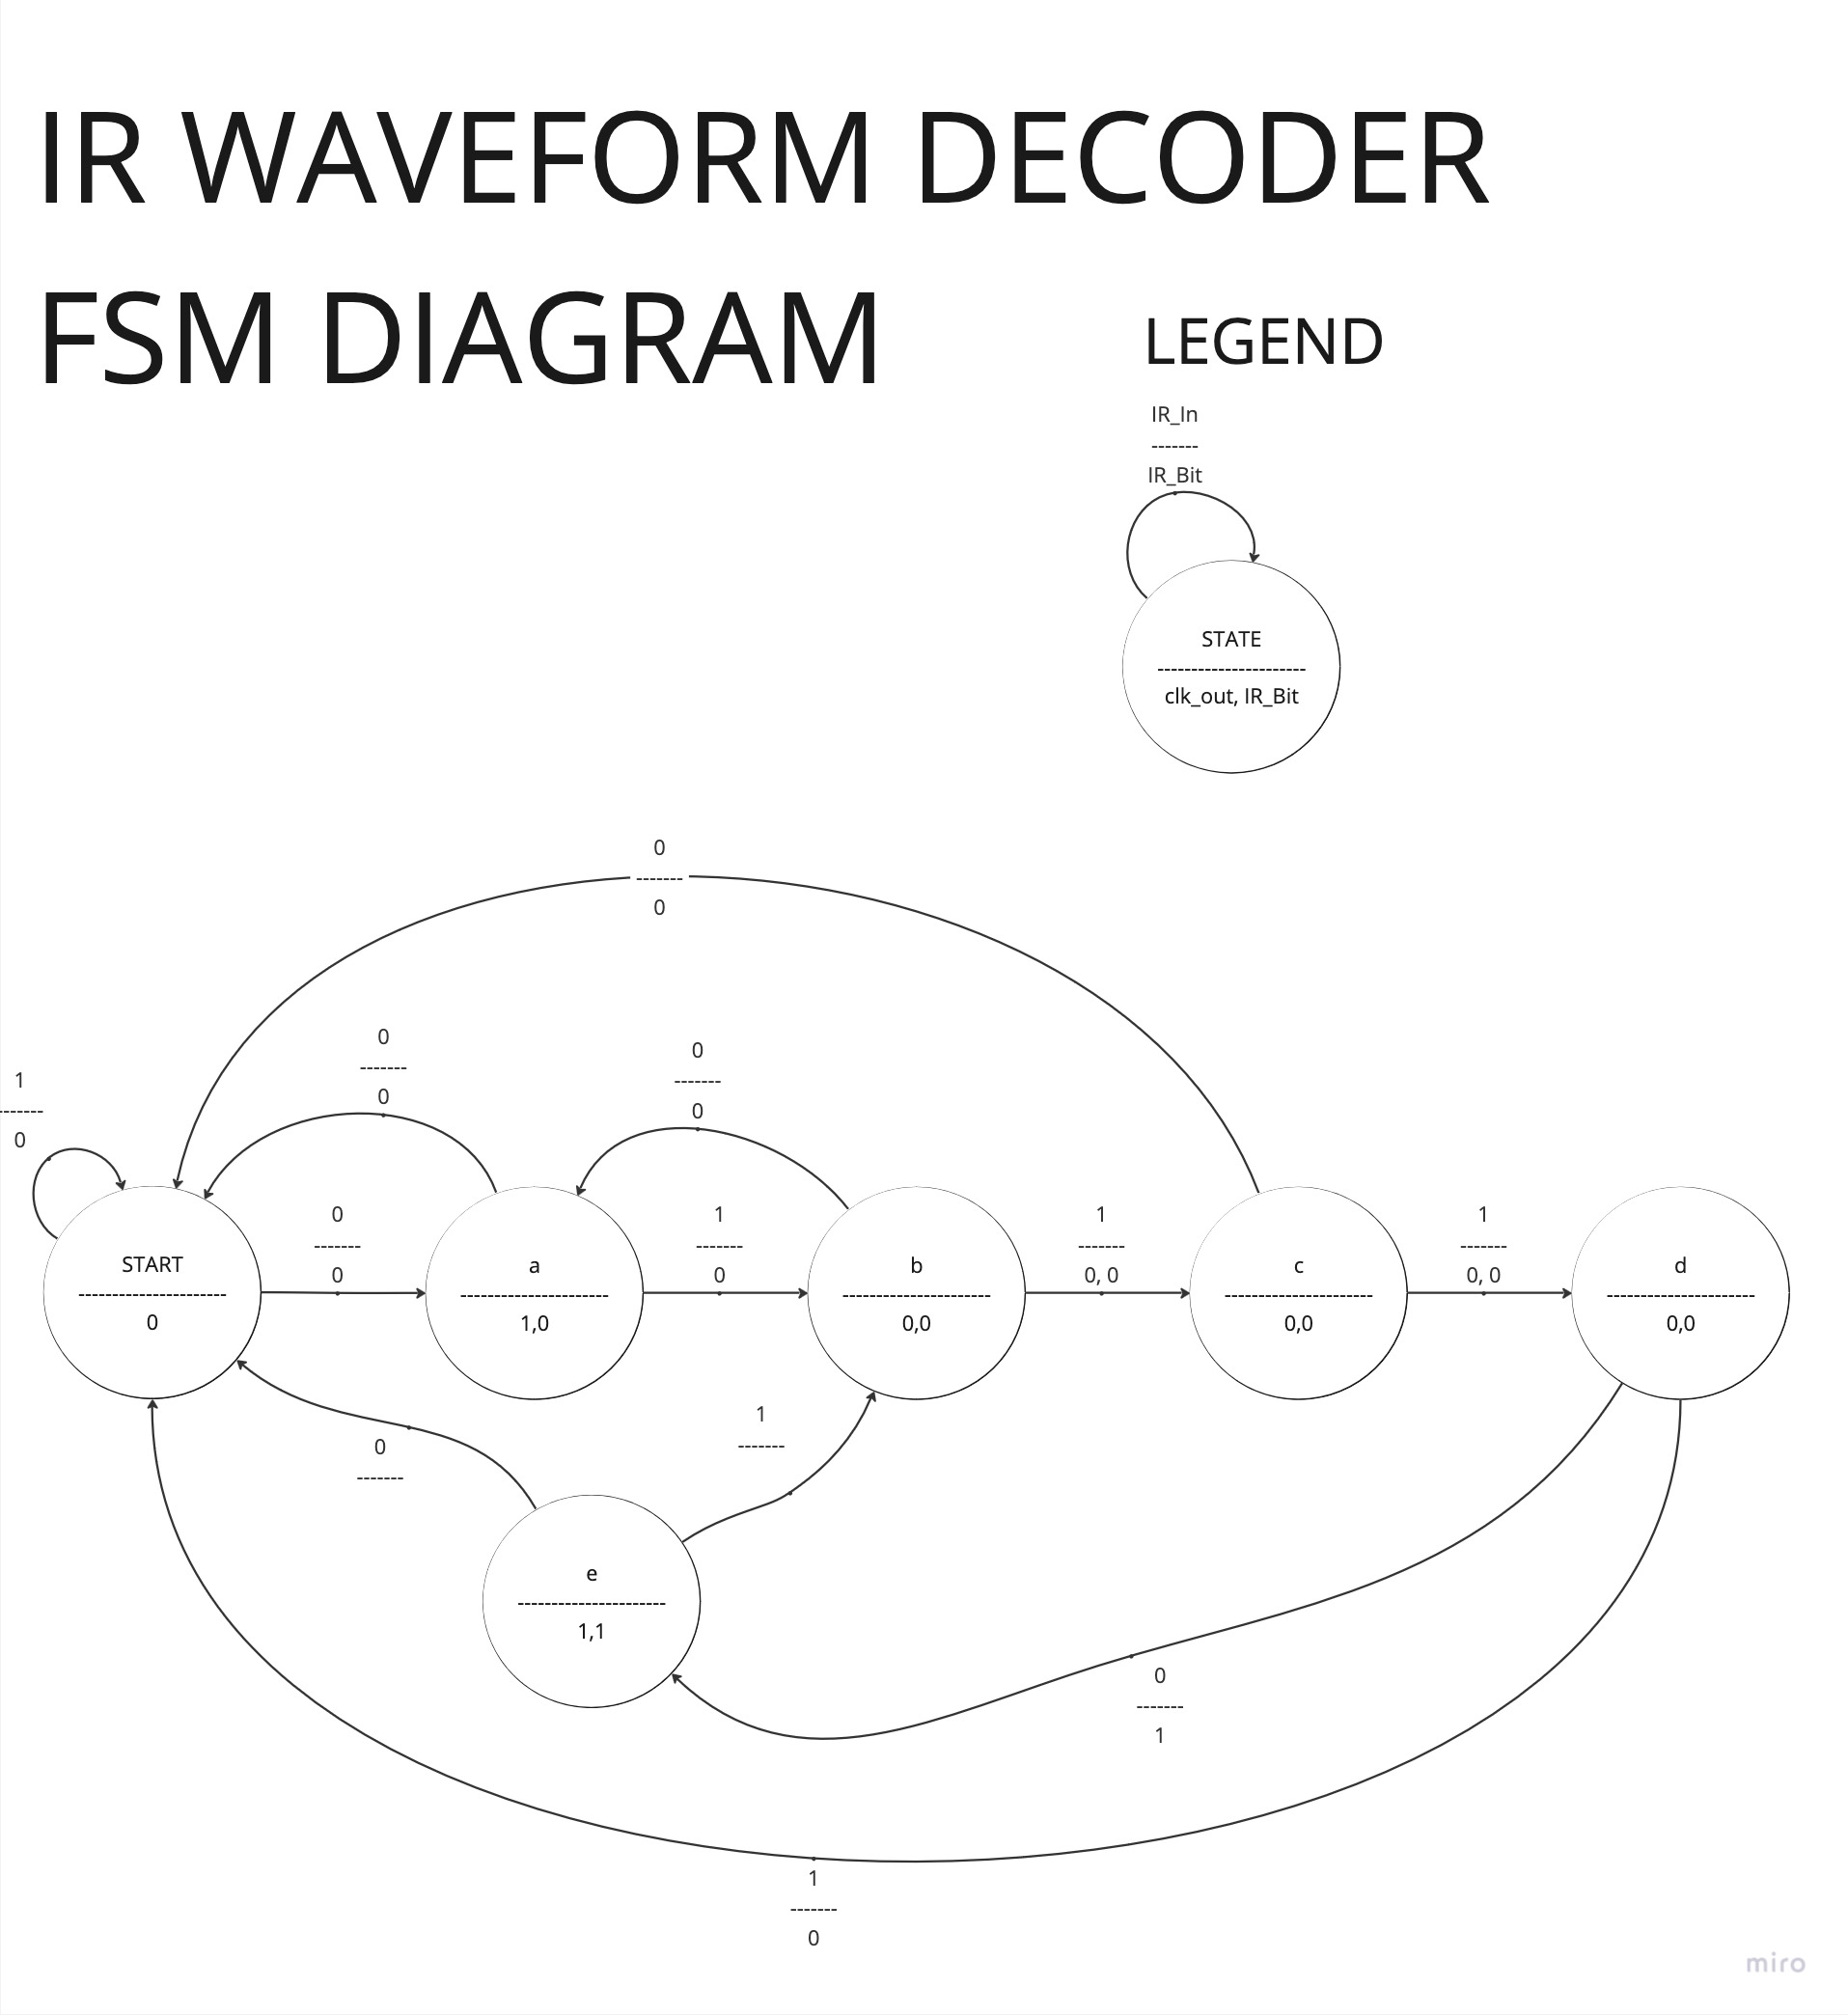
\includegraphics[width=.8\textwidth]{Figures/FSM Decoder Diagram.jpg}
        \caption{State Diagram of first “waveform decoder” FSM}
        \label{fig:lowlevelblockdiagram}
    \end{figure}

    \begin{figure}[h]
        \centering
        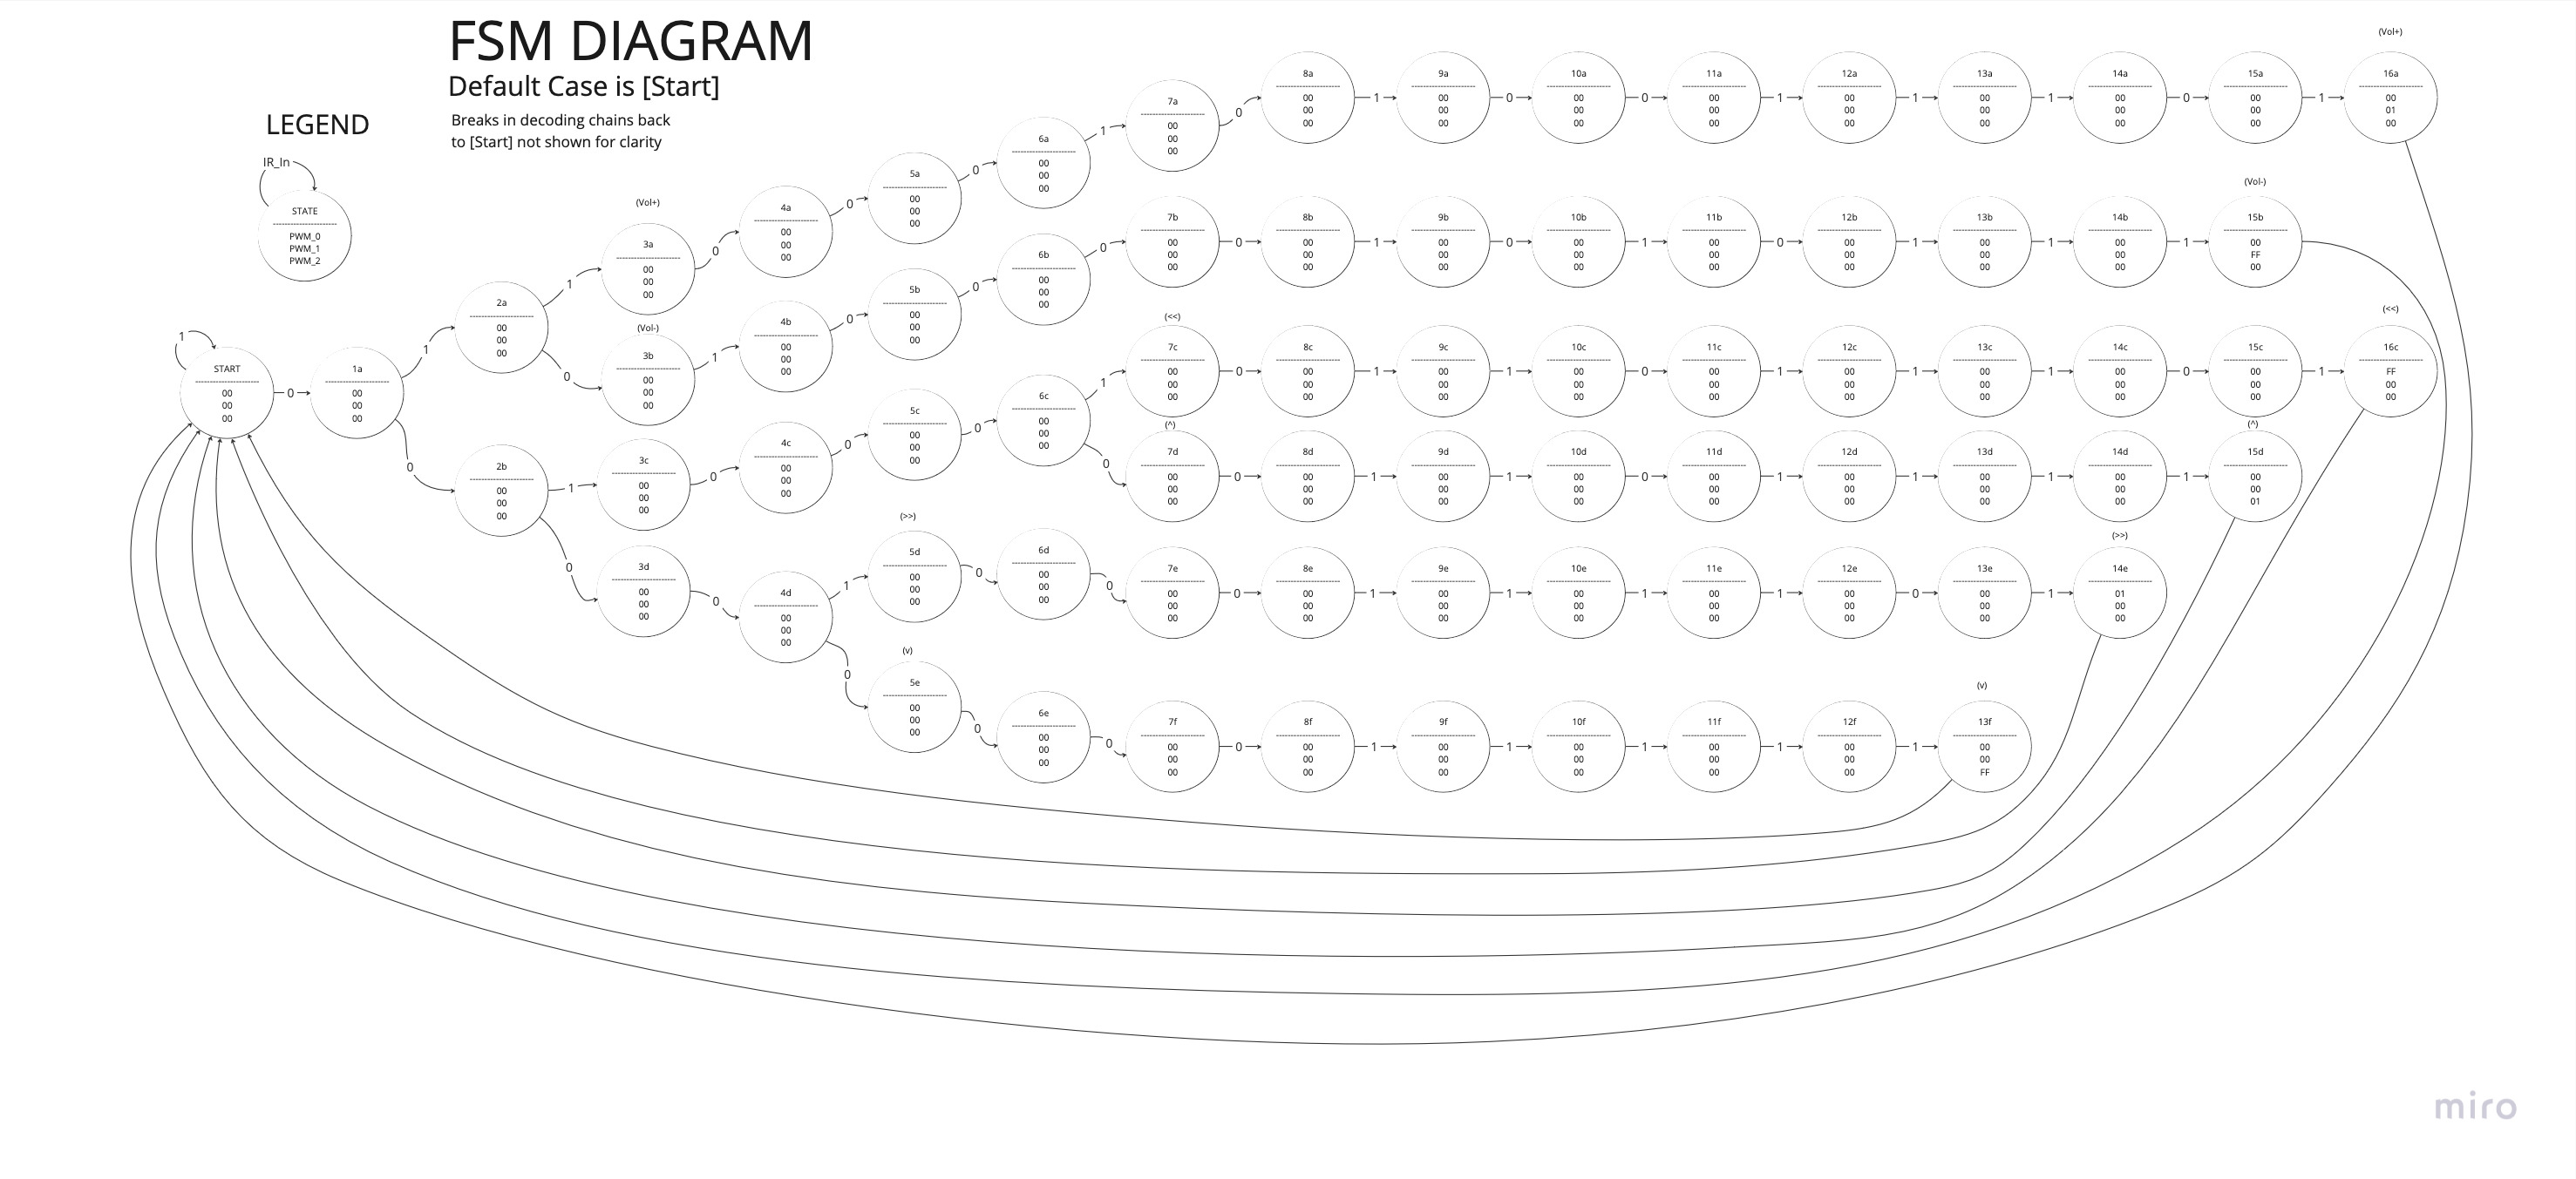
\includegraphics[width=.8\pdfpagewidth]{Figures/FSM Decoder Diagram High Res.jpg}
        \caption{State Diagram of second “bitstream decoder” FSM}
        \label{fig:lowlevelblockdiagram}
    \end{figure}

    \newpage

    To time the bit processing of the IR decoding portion (The 2 FSMs), a modified version of Dr. Mealy's "Slow Clock" \verb|clock_div2.vhd| module was included, changing the clock to output 1,778 Hz frequency.

    The next portion was the data storage portion of the module, which would use an accumulator to keep a running total of each value to keep the angle of the servo motor at. A modified 8-bit accumulator was used, that added an upper and lower cap to its maximum and minimum values that could be stored, so that data overflow wouldn't happen (for instance if a -1 was entered but the value stored was 0). A decoder was added in line with the accumulator to clock pulse the second FSM to set it’s output back to 0 (since the FSM’s clock depends on the first FSM’s output, when the receiver isn’t getting data the value of the first FSM output stays constant until its clock is pulsed). The FSM after detecting the right code would output its +/- 1 into the decoder, which would be in sync with the timing of the accumulator, and would output it only once on one clock pulse to not add additional unintended data, and would also pulse the clock of the second FSM, to set it’s outputs back to low.
    
    The last portion was the PWM output section, which consisted of a second slow clock (The modified Dr. Mealy’s \verb|clock_div2.vhd|) running at a flat 1000 Hz frequency, along with a new PWM module, which would take in the stored total (representing the angle) from the accumulator, and output a PWM signal to the servo motor, corresponding to the angle the servo should be set to. The data storage and PWM sections were duplicated to a total of 3 of each line, each connecting to an output from the second FSM.


\section{Simulation and Debugging}

Our main simulation source was of the top module, which in the Vivado simulation we displayed the inner connections, showing. The 5 main linear modules worked, being the first “waveform decoder” FSM, the second “IR bitstream” FSM, and one line of the decoder, the modified accumulator, and the PWM output.

\begin{figure}[h]
    \centering
    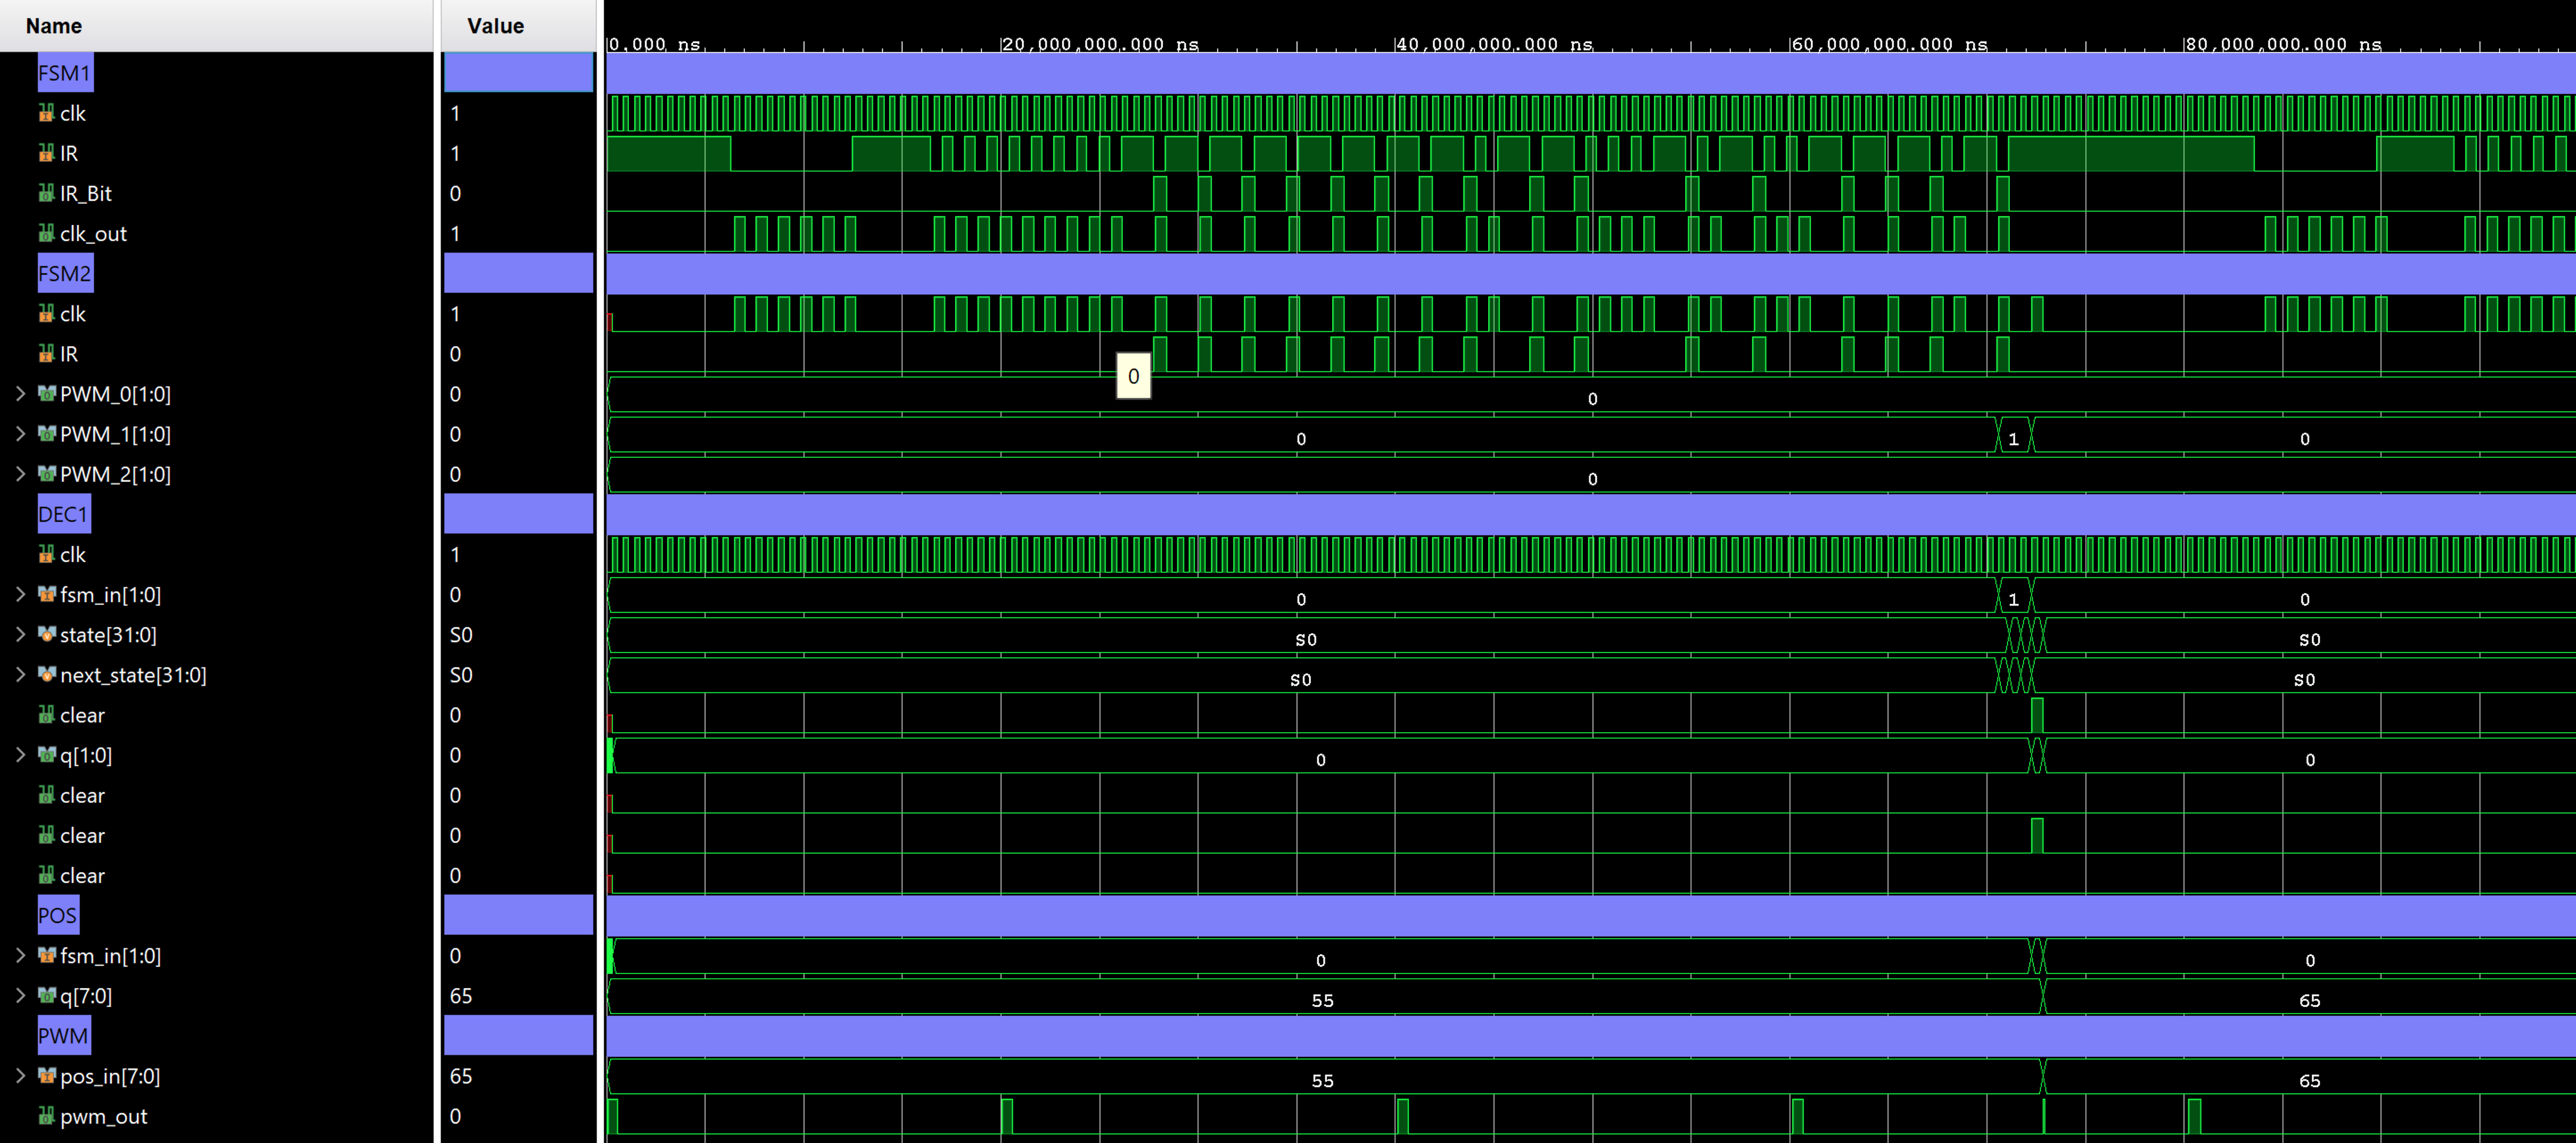
\includegraphics[width=.8\pdfpagewidth]{Figures/Final Simulation.png}
    \caption{Simulation of Robotic Arm Top Module}
    \label{fig:lowlevelblockdiagram}
\end{figure}

Our code for simulation was made by re-creating the oscilloscope output of the “VOL+” Button, making it determine the timing diagram for our only input, the IR input. We then simulated the output of the corresponding \verb|PWM_1| line, showing that its Pulse Width duty cycle changed with each button press, and therefore each correct bitstream of data. Our simulation output is shown above, as well as our simulation code is shown below. 

\newpage
\subsection{Simulation Code}
\begin{lstlisting}[language=VHDL]
    `timescale 1ns / 1ps
////////////////////////////////////////////////////////////
// Company: Cal Poly SLO   
// Engineer: Wyatt Tack
// 
// Create Date: 11/29/2023 01:59:28 PM
// Design Name: Robot Arm Test Bench
// Module Name: FSM_TB
// Project Name: Robotic Arm
// Target Devices: Basys 3 Development Board
// Tool Versions: 
// Description: 
// 
// Dependencies: 
// 
// Revision:
// Revision 0.01 - File Created
// Additional Comments:
// 
////////////////////////////////////////////////////////////


module FSM_TB();
logic clk;
logic IR;
logic PWM_0, PWM_1, PWM_2;

Robot_Arm UUT (.clk(clk), .IR(IR), .PWM_0(PWM_0), .PWM_1(PWM_1), .PWM_2(PWM_2));

always begin//100 MHz, 10ns Period
clk = 1;
#5;
clk = 0;
#5;
end

always begin
IR = 1;
#6287500;

IR = 0;
#6187500;

IR = 1;
#3937500;

IR = 0;
#600000; 

IR = 1; //0
#536000; 
IR = 0;
#600000; 

IR = 1; //0
#536000; 
IR = 0;
#600000; 

IR = 1; //0
#536000; 
IR = 0;
#600000; 

IR = 1; //0
#536000; 
IR = 0;
#600000; 

IR = 1; //0
#536000; 
IR = 0;
#600000; 

IR = 1; //0
#536000; 
IR = 0;
#600000; 

IR = 1; //0
#536000; 
IR = 0;
#600000; 

IR = 1; //0
#536000; 
IR = 0;
#600000;

IR = 1; //1
#1644000; 
IR = 0;
#600000;

IR = 1; //1
#1644000; 
IR = 0;
#600000;

IR = 1; //1
#1644000; 
IR = 0;
#600000;

IR = 1; //1
#1644000; 
IR = 0;
#600000;

IR = 1; //1
#1644000; 
IR = 0;
#600000;

IR = 1; //1
#1644000; 
IR = 0;
#600000;

IR = 1; //1
#1644000; 
IR = 0;
#600000;

IR = 1; //1
#1644000; 
IR = 0;
#600000;

//initializer ^^^
IR = 1; //0
#536000; 
IR = 0;
#600000;

IR = 1; //1
#1644000; 
IR = 0;
#600000;

IR = 1; //1
#1644000; 
IR = 0;
#600000;

IR = 1; //0
#536000; 
IR = 0;
#600000;

IR = 1; //0
#536000; 
IR = 0;
#600000;

IR = 1; //0
#536000; 
IR = 0;
#600000;

IR = 1; //1
#1644000; 
IR = 0;
#600000;

IR = 1; //0
#536000; 
IR = 0;
#600000;

IR = 1; //1
#1644000; 
IR = 0;
#600000;

IR = 1; //0
#536000; 
IR = 0;
#600000;

IR = 1; //0
#536000; 
IR = 0;
#600000;

IR = 1; //1
#1644000; 
IR = 0;
#600000;

IR = 1; //1
#1644000; 
IR = 0;
#600000;

IR = 1; //1
#1644000; 
IR = 0;
#600000;

IR = 1; //0
#536000; 
IR = 0;
#600000;

IR = 1; //1
#1644000; 
IR = 0;
#600000;

//end code^^^
IR=1;
#6187500;
end
endmodule


\end{lstlisting}
    


\section{Implemented Code}


Our final code consisted of one top module, 2 FSMs, 2 Modified Dr. Mealy modules, A Modified Accumulator, a new Decoder, and a new PWM Module, resulting in 3 modified Modules and 5 brand new Low Level Modules. The code is shown below, modified modules first, then everything else in order of hierarchy and flow of data. All code can be additionally found at the following Github link:
\\ \url{ https://github.com/EthanV1920/CPE-133-Final-Lab}

\subsection{Slow Clock Module 1}

Only changed line 38 to change the frequency of the clock.

\begin{lstlisting}[language=VHDL]
-- Only line(38) changed is the MAX_COUNT constant
constant max_count : integer := (28124);
\end{lstlisting}


\subsection{Slow Clock Module 2}

Only changed line 38 to change the frequency of the clock.

\begin{lstlisting}[language=VHDL]
-- Only line(38) changed is the MAX_COUNT constant
constant max_count : integer := (500);
\end{lstlisting}

\subsection{Modified Accumulator}

Ethan Vosburg modified the accumulator to add an upper and lower cap to its maximum and minimum values that could be stored, so that data overflow wouldn't happen (for instance if a -1 was entered but the value stored was 0). The code is shown below.

\begin{lstlisting}[language=VHDL]
    
module POS_ACC(
    // Inputs
    input [1:0] fsm_in, // Signed 2bit input
    input clk, ld, clear, // Clock, load, and clear inputs

    // Outputs
    output logic [7:0] q = 8'd55 // Accumulator output
    );
    
    // Accumulator Logic
    always_ff @ (posedge clk)
    begin
        if (clear)
            begin
                // Reset the accumulator
                q <= 8'd55;
            end 
        else if (ld)
            // Increment the accumulator when load is +1
            // $display("q = %d", q); // Debug code
            if ((q >= 8'd55) && (q <= 8'd245))
                begin    
                    if (fsm_in == 2'b01)
                        begin 
                            q <= q + 8'd10;
                        end
                end
            // Decerement the accumulator when load is -1
            if ((q >= 8'd65) && (q <= 8'd255))
                if (fsm_in == 2'b11)
                    q <= q - 8'd10;
    end

endmodule
\end{lstlisting}

\subsection{Top Module}

\begin{lstlisting}[language=VHDL]
    `timescale 1ns / 1ps
/////////////////////////////////////////////////////////////////////
// Company: Cal Poly SLO
// Engineer: Ethan Vosburg and Wyatt Tack
// 
// Create Date: 11/29/2023 02:09:10 PM
// Design Name: Robot Arm Top Module
// Module Name: Robot_Arm
// Project Name: Robotic Arm
// Target Devices: Baysys 3 Development Board
// Tool Versions: 
// Description: Top module for the robotic arm linking all modules together
// 
// Dependencies: 
// 
// Revision: 1.0
// Revision 0.01 - File Created
// Additional Comments:
// 
/////////////////////////////////////////////////////////////////////


module Robot_Arm(
    // Input Ports
    input clk,
    input IR,

    // Output Ports
    output PWM_0, PWM_1, PWM_2,
    output PWR, GND,

    // Debug Ports
    output debug_0, debug_1, debug_2, debug_3, debug_4, debug_5
    );
logic SCLK_0, IR_BIT, FSM_CLK_IN, FSM_CLK_OUT; 
logic DEC_CLR_0, DEC_CLR_1, DEC_CLR_2;
logic [1:0] FSM_DEC_0, FSM_DEC_1, FSM_DEC_2;
logic [1:0] ACC_0, ACC_1, ACC_2;
logic [7:0] ACC_0_PWM_0, ACC_1_PWM_1, ACC_2_PWM_2;
logic debug_led_0, debug_led_1, debug_led_2;


assign PWR = 1;
assign GND = 0;

assign FSM_CLK_IN = FSM_CLK_OUT | DEC_CLR_0 | DEC_CLR_1 | DEC_CLR_2;

clk_div2_0 SCLK_D_0 (
    .clk(clk),
    .sclk(SCLK_0)
    );

clk_div2_1 SCLK_D_1 (
    .clk(clk),
    .sclk(SCLK_1)
    );

FSM_Decoder FSM1 (
    .clk(SCLK_0),
    .IR(IR),
    .IR_Bit(IR_BIT),
    .clk_out(FSM_CLK_OUT)
    );


FSM_IR FSM2 (
    .clk(FSM_CLK_IN),
    .IR(IR_BIT),
    .PWM_0(FSM_DEC_0),
    .PWM_1(FSM_DEC_1),
    .PWM_2(FSM_DEC_2)
    );

assign debug_0 = FSM_CLK_OUT;
assign debug_1 = FSM_CLK_IN;
assign debug_2 = DEC_CLR_2;
assign debug_3 = FSM_DEC_2[0];
assign debug_4 = DEC_CLR_2;
assign debug_5 = FSM_DEC_2[0];



DEC DEC_0 (
    .fsm_in(FSM_DEC_0),
    .clk(SCLK_0),
    .q(ACC_0),
    .clear(DEC_CLR_0)
    );

// assign debug_0 = ACC_0[0];
// assign debug_1 = ACC_0[1];

DEC DEC_1 (
    .fsm_in(FSM_DEC_1),
    .clk(SCLK_0),
    .q(ACC_1),
    .clear(DEC_CLR_1)
    );

// assign debug_2 = ACC_1[0];
// assign debug_3 = ACC_1[1];

DEC DEC_2 (
    .fsm_in(FSM_DEC_2),
    .clk(SCLK_0),
    .q(ACC_2),
    .clear(DEC_CLR_2)
    );

// assign debug_4 = ACC_2[0];
// assign debug_5 = ACC_2[1];

POS_ACC POS_ACC_0 (
    .fsm_in(ACC_0),
    .clk(SCLK_0),
    .clear(1'b0),
    .ld(1'b1),
    .q(ACC_0_PWM_0)
    );

POS_ACC POS_ACC_1 (
    .fsm_in(ACC_1),
    .clk(SCLK_0),
    .clear(1'b0),
    .ld(1'b1),
    .q(ACC_1_PWM_1)
    );

POS_ACC POS_ACC_2 (
    .fsm_in(ACC_2),
    .clk(SCLK_0),
    .clear(1'b0),
    .ld(1'b1),
    .q(ACC_2_PWM_2)
    );

PWM PWM_D_0 (
    .clk(SCLK_1),
    .pos_in(ACC_0_PWM_0),
    .pwm_out(PWM_0)
    );

PWM PWM_D_1 (
    .clk(SCLK_1),
    .pos_in(ACC_1_PWM_1),
    .pwm_out(PWM_1)
    );

PWM PWM_D_2 (
    .clk(SCLK_1),
    .pos_in(ACC_2_PWM_2),
    .pwm_out(PWM_2)
    );
    
endmodule
\end{lstlisting}

\newpage

\subsection{FSM Module 1}

\begin{lstlisting}[language=VHDL]
`timescale 1ns / 1ps
/////////////////////////////////////////////////////////////////////
// Company: Cal Poly SLO
// Engineer: Wyatt Tack
// 
// Create Date: 12/01/2023 02:14:47 PM
// Design Name: FSM IR NEC decoder
// Module Name: FSM_Decoder
// Project Name: IR controlled robotic arm
// Target Devices: Elegoo IR Remote and reciever module
// Tool Versions: 
// Description: Uses an FSM to decode the output of an NEC protocol IR module to
//              Determine if the output is a 1 or a 0 bit   
//
// Dependencies: Slow Clock 1 (1778 HZ)
// 
// Revision:
// Revision 0.01 - File Created
// Additional Comments:
// 
/////////////////////////////////////////////////////////////////////
    
    
    module FSM_Decoder(
        // Inputs
        input clk, // Clock input
        input IR, // IR input
    
        // Outputs
        output logic IR_Bit, // IR output logic
        output logic clk_out // Clock output logic
        );
    
        // Defined states for delay
        typedef enum {Start, a, b, c, d, e} STATES;
        
        // Defines the current and next state
        STATES PS, NS;
    
        // Clock logic
        always_ff@(posedge clk)
        begin
            PS <= NS;
        end   
        
        // State logic
        always_comb
        begin
            // Set IR_Bit and clk_out to 0
            IR_Bit = 0;
            clk_out = 0;
        case (PS)
            Start:
            begin
            clk_out = 0;
            if (IR) 
            begin
            NS = Start;
            IR_Bit = 0;
            end
            else 
            begin
            NS = a;
            IR_Bit = 0;
            end
            end
            a:
            begin
            clk_out = 1;
            if (IR) 
                begin
                NS = b;
                IR_Bit = 0;
                end
            else 
                begin
                NS = Start;
                IR_Bit = 0;
                end
            end
            b:
            begin
            clk_out = 0;
            if (IR) 
                begin
                NS = c;
                IR_Bit = 0;
                end
            else 
                begin
                NS = a;
                IR_Bit = 0;
                end
            end
            c:
            begin
            clk_out = 0;
            if (IR) 
                begin
                NS = d;
                IR_Bit = 0;
                end
            else 
                begin
                NS = Start;
                IR_Bit = 0;
                end
            end
            d:
            begin
            clk_out = 0;
            if (IR) 
                begin
                NS = Start;
                IR_Bit = 0;
                end
            else 
                begin
                NS = e;
                IR_Bit = 1;
                end
            end
            e:
            begin
            clk_out = 1;
            IR_Bit = 1;
            if (IR) 
                begin
                NS = b;
                //IR_Bit = 0;
                end
            else 
                begin
                NS = Start;
                //IR_Bit = 0;
                end
            end
            
            
        default:
        NS = Start;
        endcase
        end   
    endmodule
\end{lstlisting}    

\subsection{FSM Module 2}

\begin{lstlisting}[language=VHDL]

`timescale 1ns / 1ps
/////////////////////////////////////////////////////////////////////
// Company: Cal Poly SLO
// Engineer: Wyatt Tack
// 
// Create Date: 11/28/2023 10:26:21 AM
// Design Name: IR FSM Decoder
// Module Name: FSM_IR
// Project Name: Remote Control Servo Arm
// Target Devices: Elegoo IR remote and receiver module
// Tool Versions: 
// Description: Uses an FSM to decode a 38kHz IR signal from a remote, 
//              to add +/- 1 to a variable controlling the position of a servo motor
// 
// Dependencies: FSM IR Bit Decoder
// 
// Revision: 1.0
// Revision 0.01 - File Created
// Additional Comments:
// 
/////////////////////////////////////////////////////////////////////


module FSM_IR(
    // Inputs
    input clk, // Clock input
    input IR, // IR input

    // Outputs
    output logic [1:0] PWM_0, PWM_1, PWM_2 // PWM outputs
    );
    
    // Define states
    typedef enum {Start, a1, a2, a3, a4, a5, a6, a7, a8, a9, a10, a11, a12, a13, a14, a15, a16, 
    b2, b3, b4, b5, b6, b7, b8, b9, b10, b11, b12, b13, b14, b15, 
    c3, c4, c5, c6, c7, c8, c9, c10, c11, c12, c13, c14, c15, c16, 
    d3, d4, d5, d6, d7, d8, d9, d10, d11, d12, d13, d14, d15, 
    e5, e6, e7, e8, e9, e10, e11, e12, e13, e14, 
    f7, f8, f9, f10, f11, f12, f13} STATES;
    
    // Define current and next state
    STATES PS, NS;
    

    // Clock logic
    always_ff@(posedge clk)
    begin
    PS <= NS;
    end
    
    // FSM logic
    always_comb
    begin
    PWM_0 = 0;
    PWM_1 = 0;
    PWM_2 = 0;
    case (PS)
        Start://11111...
        begin
        PWM_0 = 0;
        PWM_1 = 0;
        PWM_2 = 0;
        if (IR) NS = Start;
        else NS = a1;
        end
        a1://0
        begin
        if (IR) NS = a2;
        else NS = b2;
        end
        a2://01
        begin
        if (IR) NS = a3;
        else NS = b3;
        end
        a3://011
        begin
        if (!IR) NS = a4;
        else NS = Start;
        end
        a4://0110
        begin
        if (!IR) NS = a5;
        else NS = Start;
        end 
        a5://01100
        begin
        if (!IR) NS = a6;
        else NS = Start;
        end
        a6://011000
        begin
        if (IR) NS = a7;
        else NS = Start;
        end
        a7://0110001
        begin
        if (!IR) NS = a8;
        else NS = Start;
        end
        a8://01100010
        begin
        if (IR) NS = a9;
        else NS = Start;
        end
        a9://011000101
        begin
        if (!IR) NS = a10;
        else NS = Start;
        end
        a10://0110001010
        begin
        if (!IR) NS = a11;
        else NS = Start;
        end
        a11://01100010100
        begin
        if (IR) NS = a12;
        else NS = Start;
        end
        a12://011000101001
        begin
        if (IR) NS = a13;
        else NS = Start;
        end
        a13://0110001010011
        begin
        if (IR) NS = a14;
        else NS = Start;
        end
        a14://01100010100111
        begin
        if (!IR) NS = a15;
        else NS = Start;
        end
        a15://011000101001110
        begin
        if (IR) NS = a16;
        else NS = Start;
        end
        a16://0110001010011101
        begin
        PWM_1 = 2'b01;
        NS = Start;
        end
        b2://00
        begin
        if (IR) NS = c3;
        else NS = d3;
        end
        b3://010
        begin
        if (IR) NS = b4;
        else NS = Start;
        end
        b4://0101
        begin
        if (!IR) NS = b5;
        else NS = Start;
        end
        b5://01010
        begin
        if (!IR) NS = b6;
        else NS = Start;
        end
        b6://010100
        begin
        if (!IR) NS = b7;
        else NS = Start;
        end
        b7://0101000
        begin
        if (!IR) NS = b8;
        else NS = Start;
        end
        b8://01010000
        begin
        if (IR) NS = b9;
        else NS = Start;
        end
        b9://010100001
        begin
        if (!IR) NS = b10;
        else NS = Start;
        end
        b10://0101000010
        begin
        if (IR) NS = b11;
        else NS = Start;
        end
        b11://01010000101
        begin
        if (!IR) NS = b12;
        else NS = Start;
        end
        b12://010100001010
        begin
        if (IR) NS = b13;
        else NS = Start;
        end
        b13://0101000010101
        begin
        if (IR) NS = b14;
        else NS = Start;
        end
        b14://01010000101011
        begin
        if (IR) NS = b15;
        else NS = Start;
        end
        b15://010100001010111
        begin
        PWM_1 = 2'b11;
        NS = Start;
        end
        c3://001
        begin
        if (!IR) NS = c4;
        else NS = Start;
        end
        c4://0010
        begin
        if (!IR) NS = c5;
        else NS = Start;
        end
        c5://00100
        begin
        if (!IR) NS = c6;
        else NS = Start;
        end
        c6://001000
        begin
        if (IR) NS = c7;
        else NS = d7;
        end
        c7://0010001
        begin
        if (!IR) NS = c8;
        else NS = Start;
        end
        c8://00100010
        begin
        if (IR) NS = c9;
        else NS = Start;
        end
        c9://001000101
        begin
        if (IR) NS = c10;
        else NS = Start;
        end
        c10://0010001011
        begin
        if (!IR) NS = c11;
        else NS = Start;
        end
        c11://00100010110
        begin
        if (IR) NS = c12;
        else NS = Start;
        end
        c12://001000101101
        begin
        if (IR) NS = c13;
        else NS = Start;
        end
        c13://0010001011011
        begin
        if (IR) NS = c14;
        else NS = Start;
        end
        c14://00100010110111
        begin
        if (!IR) NS = c15;
        else NS = Start;
        end
        c15://001000101101110
        begin
        if (IR) NS = c16;
        else NS = Start;
        end
        c16://0010001011011101
        begin
        PWM_0 = 2'b11;
        NS = Start;
        end
        d3://000
        begin
        if (!IR) NS = d4;
        else NS = Start;
        end
        d4://0000
        begin
        if (IR) NS = d5;
        else NS = e5;
        end
        d5://00001
        begin
        if (!IR) NS = d6;
        else NS = Start;
        end
        d6://000010
        begin
        if (!IR) NS = e7;
        else NS = Start;
        end
        d7://0010000
        begin
        if (!IR) NS = d8;
        else NS = Start;
        end
        d8://00100000
        begin
        if (IR) NS = d9;
        else NS = Start;
        end
        d9://001000001
        begin
        if (IR) NS = d10;
        else NS = Start;
        end
        d10://0010000011
        begin
        if (!IR) NS = d11;
        else NS = Start;
        end
        d11://00100000110
        begin
        if (IR) NS = d12;
        else NS = Start;
        end
        d12://001000001101
        begin
        if (IR) NS = d13;
        else NS = Start;
        end
        d13://0010000011011
        begin
        if (IR) NS = d14;
        else NS = Start;
        end
        d14://00100000110111
        begin
        if (IR) NS = d15;
        else NS = Start;
        end
        d15://001000001101111
        begin
        PWM_2 = 2'b01;
        NS = Start;
        end
        e5://00000
        begin
        if (!IR) NS = e6;
        else NS = Start;
        end
        e6://000000
        begin
        if (!IR) NS = f7;
        else NS = Start;
        end
        e7://0000100
        begin
        if (!IR) NS = e8;
        else NS = Start;
        end
        e8://00001000
        begin
        if (IR) NS = e9;
        else NS = Start;
        end
        e9://000010001
        begin
        if (IR) NS = e10;
        else NS = Start;
        end
        e10://0000100011
        begin
        if (IR) NS = e11;
        else NS = Start;
        end
        e11://00001000111
        begin
        if (IR) NS = e12;
        else NS = Start;
        end
        e12://000010001111
        begin
        if (!IR) NS = e13;
        else NS = Start;
        end
        e13://0000100011110
        begin
        if (IR) NS = e14;
        else NS = Start;
        end
        e14://00001000111101
        begin
        PWM_0 = 2'b01;
        NS = Start;
        end
        f7://0000000
        begin
        if (!IR) NS = f8;
        else NS = Start;
        end
        f8://00000000
        begin
        if (IR) NS = f9;
        else NS = Start;
        end
        f9://000000001
        begin
        if (IR) NS = f10;
        else NS = Start;
        end
        f10://0000000011
        begin
        if (IR) NS = f11;
        else NS = Start;
        end
        f11://00000000111
        begin
        if (IR) NS = f12;
        else NS = Start;
        end
        f12://000000001111
        begin
        if (IR) NS = f13;
        else NS = Start;
        end
        f13://0000000011111
        begin
        PWM_2 = 2'b11;
        NS = Start;
        end
    default:
    NS = Start;
    endcase
    end
endmodule
\end{lstlisting}


\subsection{Decoder Module}

\begin{lstlisting}[language=VHDL]
`timescale 1ns / 1ps
/////////////////////////////////////////////////////////////////////
// Company: Cal Poly SLO
// Engineer: Ethan Vosburg
// 
// Create Date: 12/05/2023 10:14:10 PM
// Design Name: Decoder
// Module Name: DEC
// Project Name: Robotic Arm with IR input and Servo Output 
// Target Devices: Basys 3 Development Board
// Tool Versions: 
// Description: Recognizes the input from the IR FSM and passes on cycle to accumulator
// 
// Dependencies: 
// 
// Revision:
// Revision 0.01 - File Created
// Additional Comments:
// 
/////////////////////////////////////////////////////////////////////


module DEC(
    // Inputs
    input [1:0] fsm_in, // 2-bit signed input logic
    input clk, // Clock input

    // Outputs
    output logic [1:0] q, // 2-bit signed output logic
    output logic clear  // Clear output logic
    );
    
    // Defined states for delay
    typedef enum {S0, S1, S2, S3} STATES;

    // Defines the current and next state
    STATES state, next_state = S0;

    // Clock logic
    always_ff@(negedge clk) begin
        state <= next_state;
        q = 2'b00;
        clear = 1'b0;

        // State logic
        case (state)
            S2: begin
                // Set output and clear when in state 2
                if (fsm_in == 2'b01) begin
                    q = 2'b01;
                    clear = 1'b1;
                end else if (fsm_in == 2'b11) begin
                    q = 2'b11;
                    clear = 1'b1;
                end
            end
            S3: begin
                // Set output and clear when in state 3
                q = 2'b00;
                clear = 1'b0;
            end
        endcase

    end

    // Delay using state logic
    always_comb begin
        next_state = state; // Default to stay in current state
        case (fsm_in)
            2'b01:
                case (state)
                    S0: next_state = S1;
                    S1: next_state = S2;
                    S2: next_state = S3;
                    S3: next_state = S0;
                endcase
            2'b11:
                case (state)
                    S0: next_state = S1;
                    S1: next_state = S2;
                    S2: next_state = S3;
                    S3: next_state = S0;
                endcase
            default: next_state = S0;     
        endcase
    end
endmodule
\end{lstlisting}
\newpage
\subsection{PWM Module}

\begin{lstlisting}[language=VHDL]
`timescale 1ns / 1ps
/////////////////////////////////////////////////////////////////////
// Company: Cal Poly SLO
// Engineer: Ethan Vosburg
// 
// Create Date: 12/06/2023 11:32:09 PM
// Design Name: PWM Module
// Module Name: PWM
// Project Name: Robotic Arm with IR input and Servo Output 
// Target Devices: Basys 3 Development Board
// Tool Versions: 
// Description: Recive the position from the accumulator and output a PWM signal
// 
// Dependencies: 
// 
// Revision:
// Revision 0.01 - File Created
// Additional Comments:
// 
/////////////////////////////////////////////////////////////////////

    
    module PWM(
        // Inputs
        input [7:0] pos_in,
        input clk,
        // Outputs
        output logic pwm_out
        );
    
        // Registers to store the period and duty cycle
        reg [10:0] period = 0;
        reg [7:0] duty = 0;
    
        // PWM logic
        always @(posedge clk ) begin
            if (period < 11'd2000)
                begin
                    // Set pwm output high for a portion of the period
                    if (duty < pos_in)
                        begin 
                            duty <= duty + 1;
                            pwm_out <= 1;
                        end
                    else
                        begin
                            // Set pwm output low for the rest of the period
                            pwm_out <= 0;
                        end
    
                    period <= period + 1;
                end
            else
                begin
                    // Reset period and duty cycle
                    period <= 0;
                    duty <= 0;
                end
        end
    
    endmodule

\end{lstlisting}

% \end{fullwidth}

% \beg 


%----------------------------------------------------------------------------------------

\end{document}
